\subsection{NoSQL版の概要}
	2章で述べたように,医療の現場からは電子カルテや血圧計の
	出力ファイルとして様々な形式のファイルが出力される.
	この形式は医療機関が導入しているソフトに依存しているため,
	異なるソフトを導入している病院間では
	医療情報を共有することができない.
	3章のSQL版は一意のフォーマットからしか
	入力を受け付けていなかった.

	%また,電子カルテに関してはHL7で規格化されたファイルが
	%出力できることもある.


  そこで,様々なファイルでの入力を受け付ける
  Webアプリケーションを開発することをNoSQL版の第一の目標とする.

  異なる形式の入力データは同じ意味の項目であっても,
  厳密に同じ言葉を項目名にとっていないことがある.
	例えば薬を処方した日という意味の項目に対して処方日という項目名と
	日時という項目名をとっている場合がある.

  ここでは便宜的に処方日と日時のように,
	異なる項目名であるが同じ意味の項目の群を
  同義キーと呼ぶ.

  この同義キーを関連付ける機能を実装することで
	異なる形式からの入力情報を関連付ける.
  具体的な機能として,同義キーのうちのひとつが検索される際に,
  その同義キーの群の項目も検索結果として反映させることを
	第二の目標とする.

\subsection{アプリケーションの開発環境}

 Webアプリケーション開発にはjavascriptのWebフレームワークである
	Node.jsを用いた.Node.jsのパッケージであるExpressとnanoを用いた.
	ExpressはWebフレームワークで、nanoはNoSQLであるCouchDBのためのドライバである.
	その他に開発で使用したソフトを含めたバージョンなどの情報は付録に記載する.


\subsection{設計}
\subsubsection{データベース}
	CouchDBはひとつのデータベースの中に複数のドキュメントとよばれる
	データ構造を保持している.
	このドキュメントは事前にテーブルなどで定義する必要がなく,
	JSON形式であれば自由に記述できる.

	本研究ではひとつの医療行為に対してひとつのドキュメントで管理する.
	本研究で使用するドキュメントが保持する情報を表\ref{tab:doc}に示す.

	CouchDBのドキュメントのJSONの内容を図\ref{json-for-doc}に示す.
	必須の項目である\_id,\_rev以外にdata要素だけを用意した.
	今後,必要になったときに他の要素を追記することは可能である.


	\begin{figure}[htbp]
		\begin{center}
			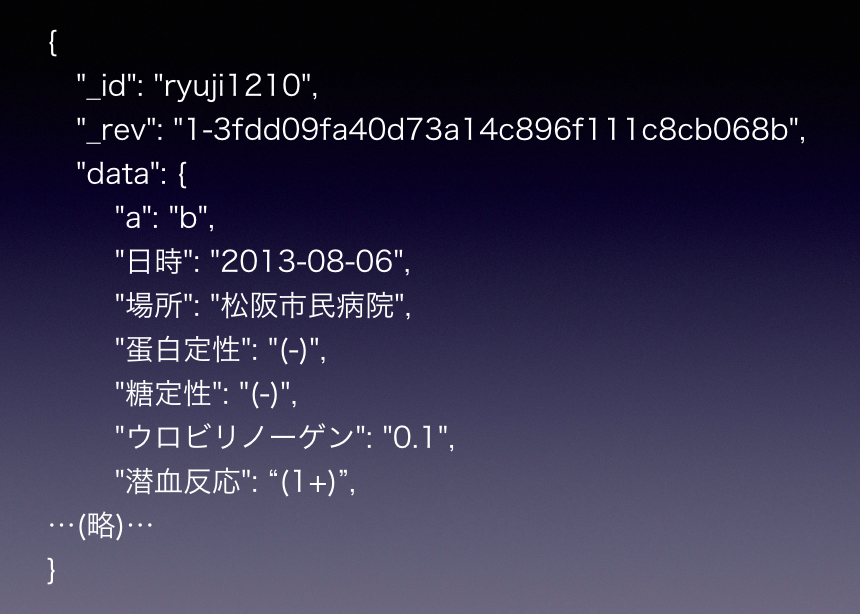
\includegraphics[width=10cm, bb=0 0 1027 737]{./gazou/json-for-doc2.png}
		\end{center}
		\caption{ドキュメントのJSONの構造}
		\label{json-for-doc}
	\end{figure}


	\begin{table}[htb]
		\begin{center}
			\caption{ドキュメントが保持する情報}
			\begin{tabular}{|l|c|r|r|}\hline
			Key & Value \\ \hline \hline
			\_id &  患者名、ドキュメント作成日をドキュメントIDとしている. \\ \hline
			\_rev & \shortstack{ドキュメントの更新回数を示す. \\ 更新時に参照し競合を防ぐ.} \\ \hline
			%name & 患者の名前 \\ \hline
			data & \shortstack{医療行為によって得られた情報を \\ json形式で格納.} \\ \hline
			\end{tabular}
			\label{tab:doc}
		\end{center}
	\end{table}


	\subsubsection{アプリケーション}
		UMLクラス図はSQL版から認可に関する機能,要素を省いたものとなる.


	\subsubsection{対応する入力ファイル}
	エクセルファイル(地域の病院で生まれるような電子化された医療情報)
	の入力に対応している.
	行と列のどちらかに日付,他方に項目があると想定して入力ファイルから
	医療情報をキーと値に関連付けてデータベースに登録していく.

	電子カルテ固有の出力ファイルはHL7に対応していれば入力ファイルから
	医療情報をキーと値に関連付けてデータベースに登録していく.
	HL7の出力ファイルはパイプ区切りで,データの並び順に意味を持たせている.
	この並び順と項目,データを関連付けてキーと値に置き直して
	データベースに登録していく.

	このとき,HL7のデータの並び順と項目の対応に関する情報が
	アプリケーション側で必要となる.



	\subsubsection{同義キーの登録}
	医療情報の出力にはキーを関連付けるためのコストがかかる.
	これは新しいフォーマットで医療情報が入力されるたびに生まれる作業となる.
	これを医療関係者にさせることを想定している.


\subsection{患者情報閲覧}

	ユーザはログイン後,Accountタブ内で検索ワードを送信すると,
	/getdbでキーに検索ワードを値に含むキーと値の組を表示する.

	ドキュメント名の日付が前後しているが,
	これはデータを入力したときの日付であるため,
	日付の順序は意味を持ってはいない.
	(図\ref{getdb})


		\begin{figure}[htbp]
			\begin{center}
				%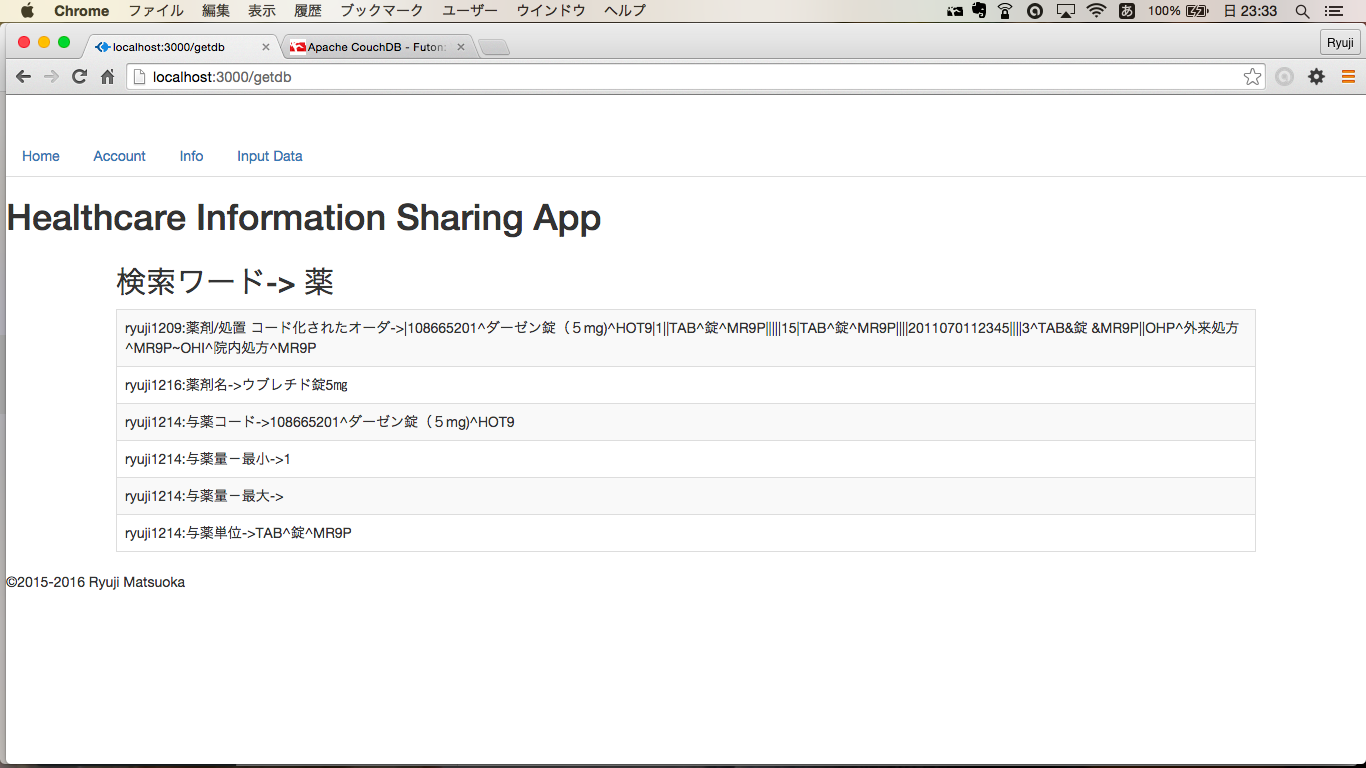
\includegraphics[width=15cm, bb=0 0 1366 1078, clip]{./gazou/getdb.png}
				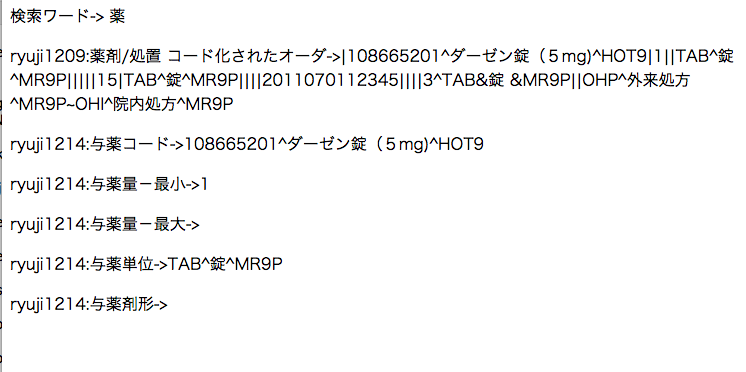
\includegraphics[width=15cm, bb=0 0 652 603, clip]{./gazou/getdb2.png}
			\end{center}
			\caption{白血球 でデータ抽出した様子}
			\label{getdb}
		\end{figure}



\subsection{データの投入方法}
	ユーザはログイン後,Input Dataタブを選択する.
	次に入力するファイルを選択し,送信する(図\ref{fileiopage}).

	\begin{figure}[htbp]
		%\begin{center}
			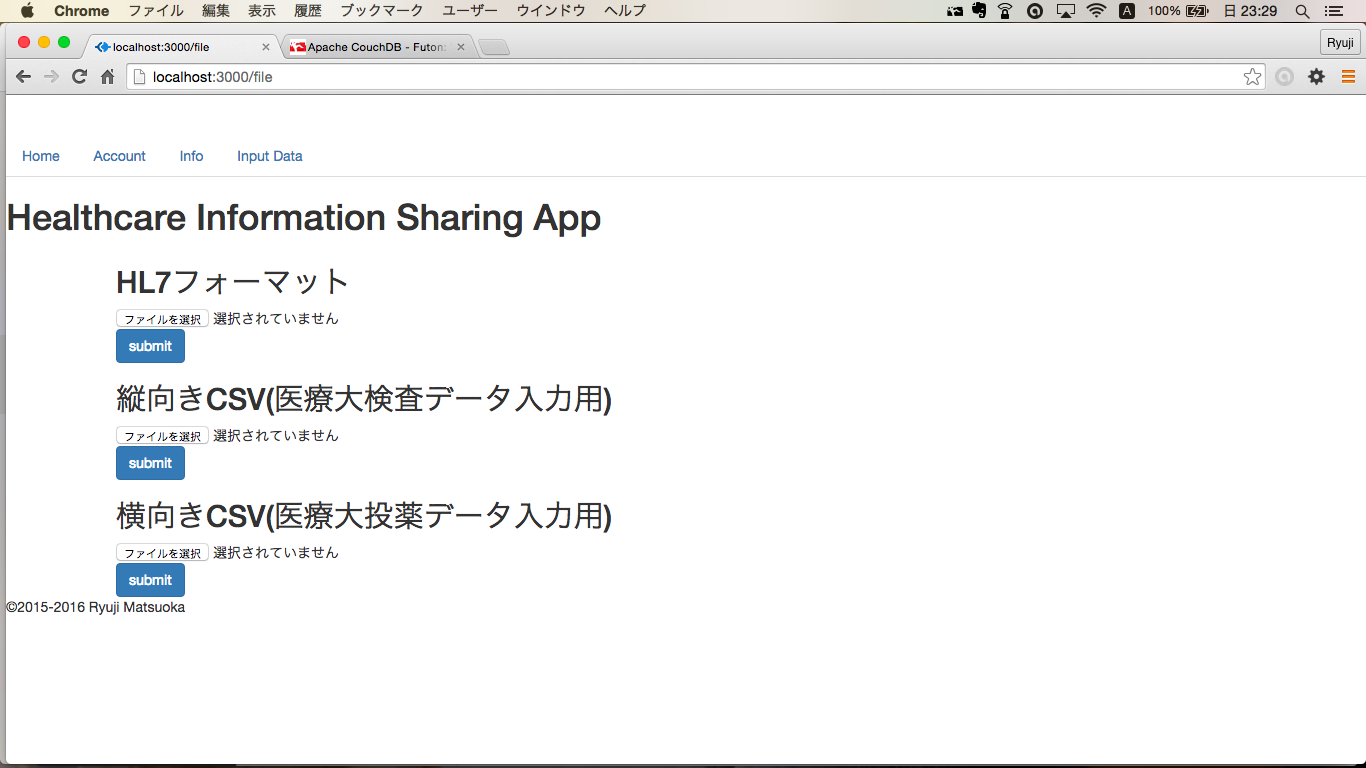
\includegraphics[width=15cm, bb=0 0 1366 1078, clip]{./gazou/fileiopage.png}
		%\end{center}
		\caption{ファイル入力ページ}
		\label{fileiopage}
	\end{figure}

	1度の診療で1つのドキュメントを生成する.
	CSV入力ファイルに複数回の診療の記録があることを許容する.

		%\subsubsection{縦向きcsvファイルの場合}
		\subsubsection{CSVファイルの場合}
			CSVファイルは入力ファイルの行,列のどちらかに医療情報,
			他方に日付をとっているものを想定している.
			図\ref{csv-data-trans}は入力内容とCouchDBへの登録内容の
			対応を表したものである.

			\begin{figure}[htbp]
				\begin{center}
					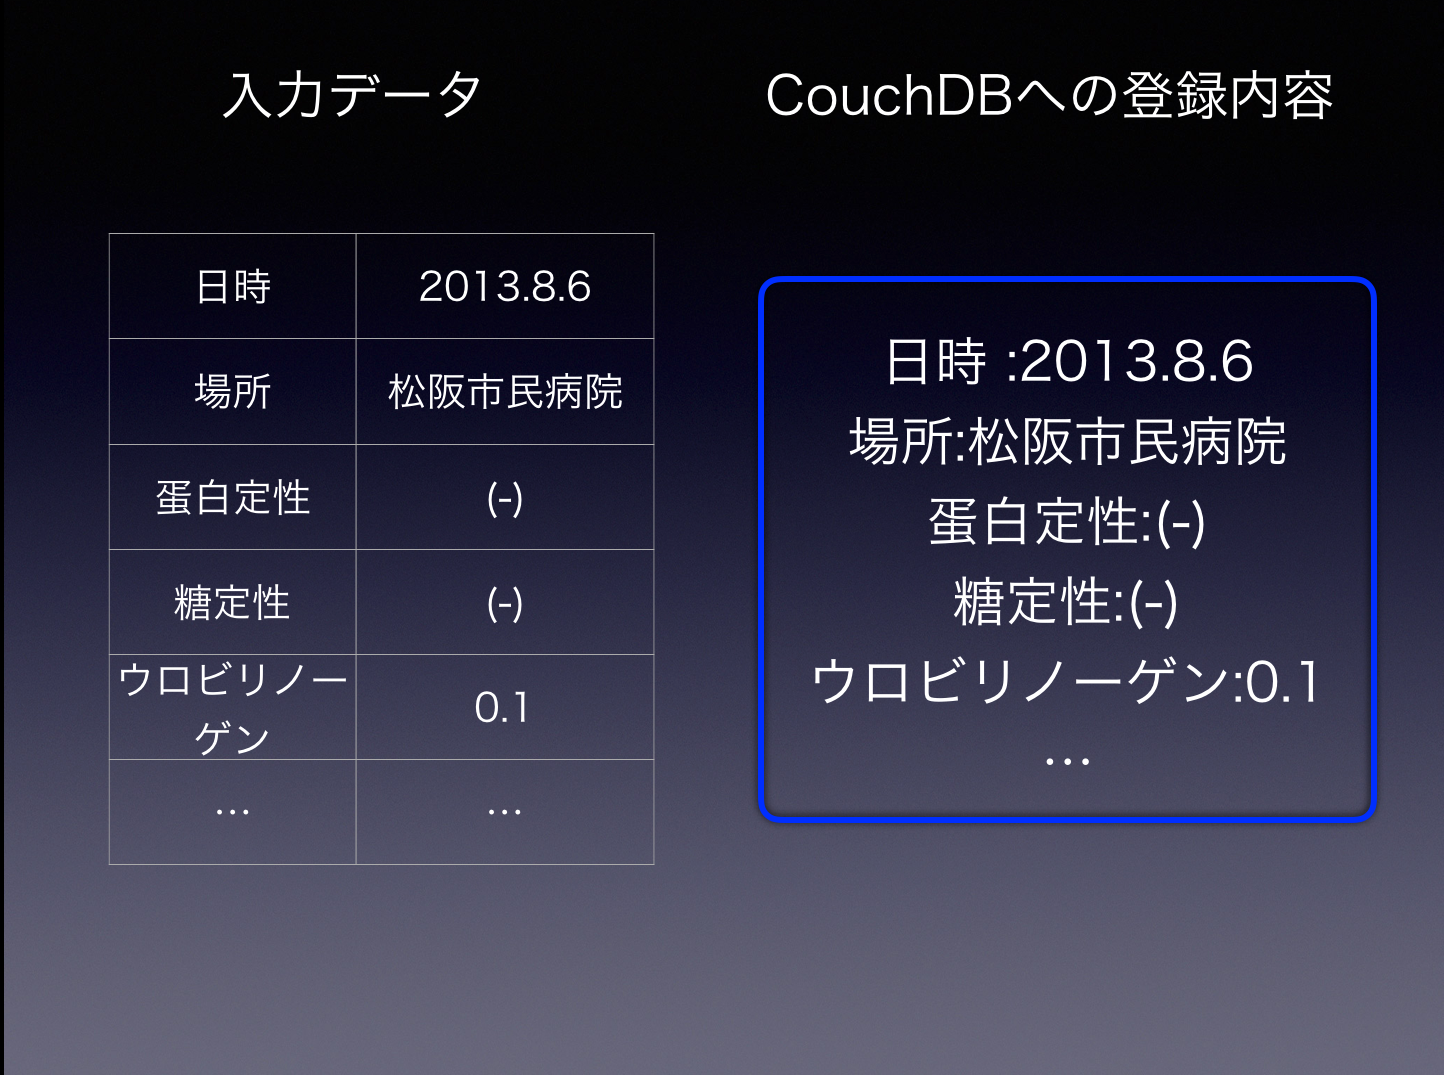
\includegraphics[width=15cm, bb=0 0 1435 1073, clip]{./gazou/csv-data-trans2.png}
				\end{center}
				\caption{入力内容とDB登録内容の対応}
				\label{csv-data-trans}
			\end{figure}

			\begin{figure}[htbp]
				\begin{center}
					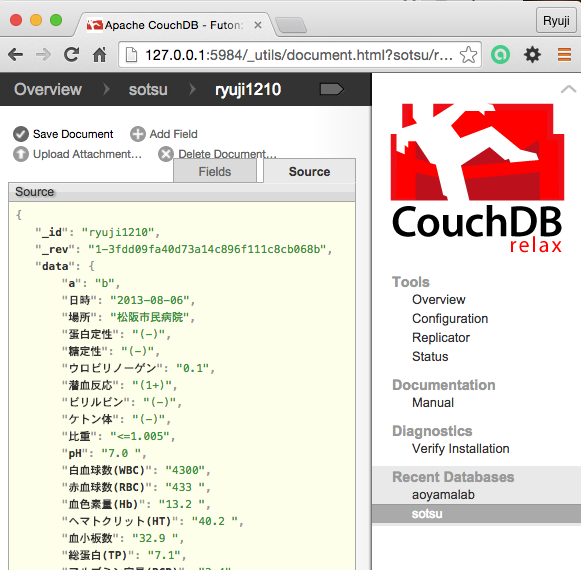
\includegraphics[width=10cm, bb=0 0 581 571, clip]{./gazou/kensa-data.png}
				\end{center}
				\caption{医療大の検査データ}
				\label{iryoudai-kensa-data}
			\end{figure}

		\if0
		\subsubsection{横向きcsvファイルの場合}
			holizontialparse
			医療大の投薬データ
		\fi


			\begin{figure}[htbp]
				\begin{center}
					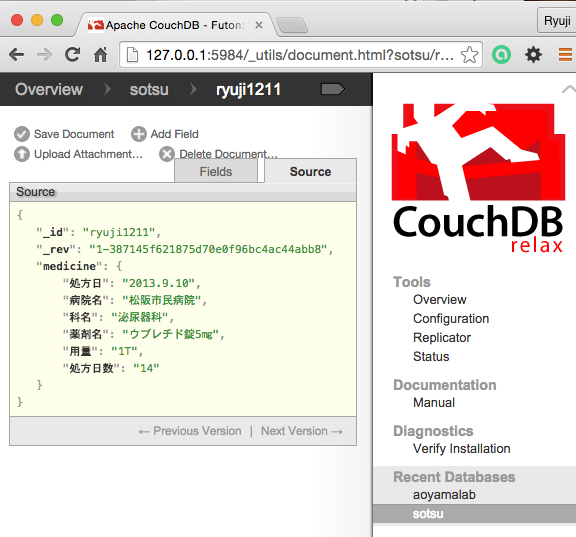
\includegraphics[width=10cm, bb=0 0 576 573]{./gazou/touyaku-data.png}
				\end{center}
				\caption{医療大の投薬データ}
				\label{iryoudai-touyaku-data}
			\end{figure}

		\subsubsection{HL7ファイルの場合}
			前述のHL7のデータ定義に基づいて入力ファイルからデータを格納していく.

			HL7の出力ファイルはパイプ区切りで記述されており,
			並び順にデータの意味が割り振られている.
			図\ref{hl7-data-trans}の枠内のデータがOBX-3という
			セグメントのデータである.
			このセグメントの意味をアプリケーション内のテーブルから参照し,
			意味とデータをJSON形式に整形してCouchDBに登録する.



			本研究では医療規格にのっとっていない医療情報との関連付けを課題としている.
			そこでHL7にのっとったファイルからデータを抜き出し,
			データの配置によって割り振られている意味をキーとしてデータベースに
			格納していく.

			\begin{figure}[htbp]
				\begin{center}
					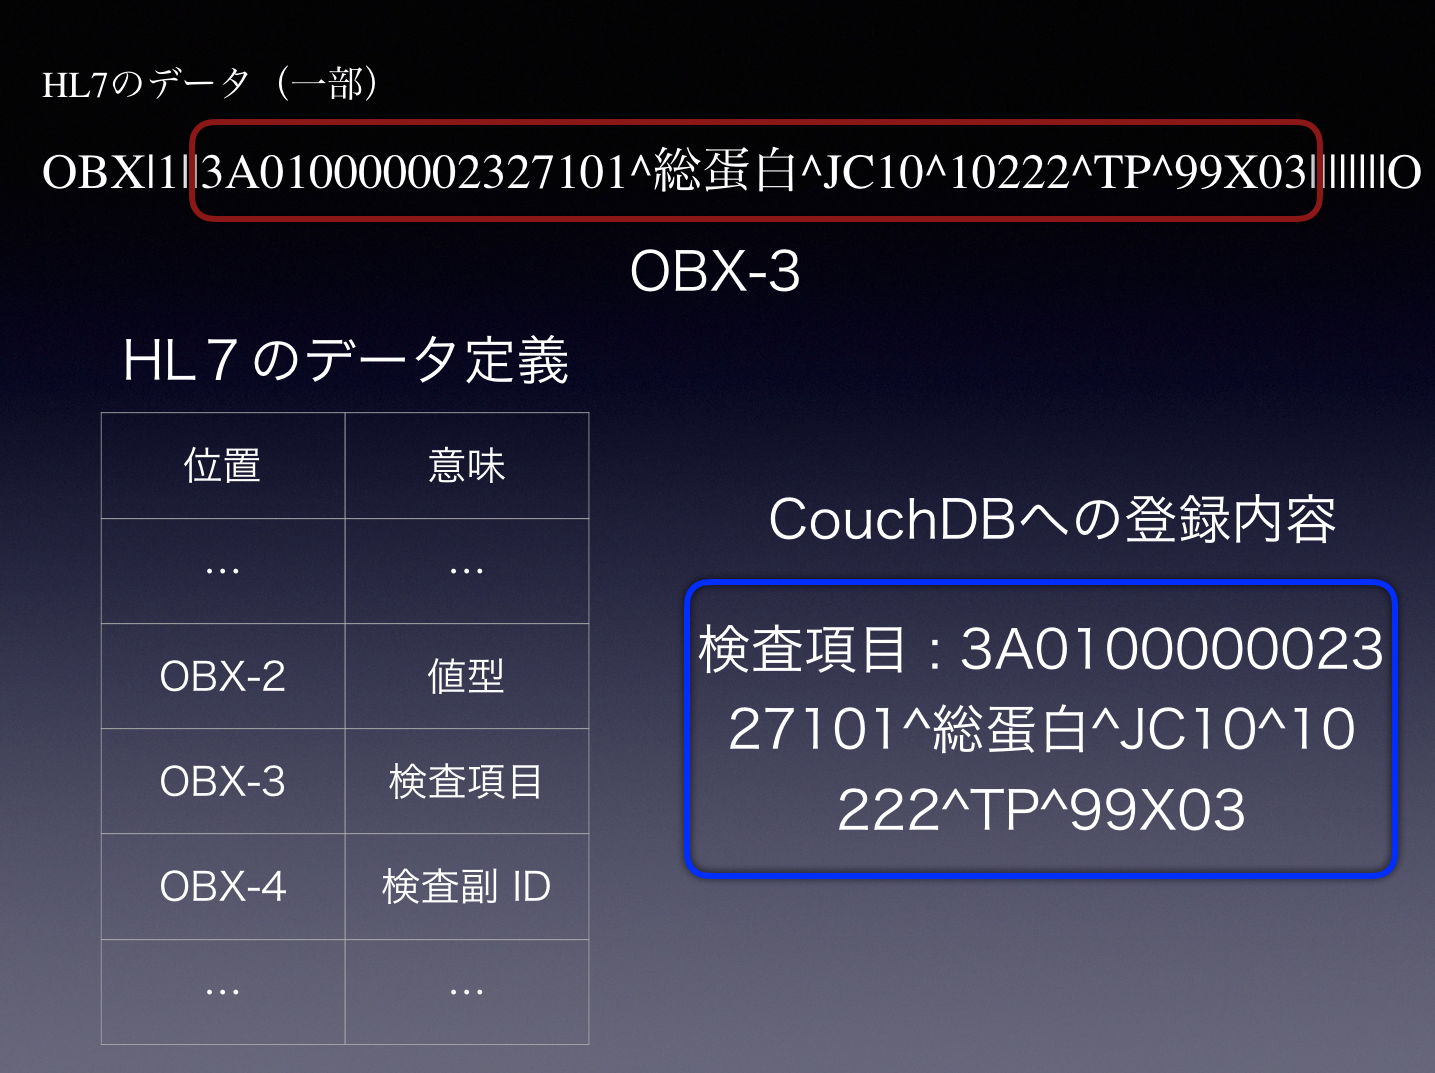
\includegraphics[width=15cm, bb=0 0 1435 1073]{./gazou/hl7-data-trans2.png}
				\end{center}
				\caption{HL7の生データからJSONへの変化}
				\label{hl7-data-trans}
			\end{figure}

			\begin{figure}[htbp]
				\begin{center}
					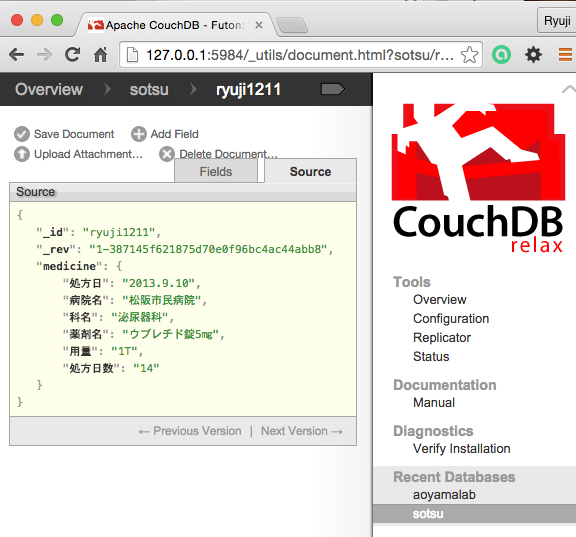
\includegraphics[width=10cm, bb=0 0 576 573]{./gazou/hl7-data.png}
				\end{center}
				\caption{HL7のサンプルデータ}
				\label{hl7-data}
			\end{figure}



\subsection{同義キーの活用}
	データを参照するときに,キーが必要となる.キーには様々な意味を持つものがあるが,
	異なる規格のデータでは同じ情報を指し示すキーであっても,
	異なるキーが使われている.
	これは新規の規格が医療情報ソフトに導入されるたびに課題となる.

	そこで,本研究ではユーザによる同義キーの登録の機能を用意した.
	ユーザは同義である2つのキーを入力すると
	それが同義キーを管理するドキュメントに追加される.

	図\ref{relation}では投薬データの処方日と診断データの日時が同義として登録されている.
	図\ref{relationApp}では検索ワードは処方であるので
	処方をキーに含むデータが検索結果として表示される.
	さらに,検索結果に処方日があり,これは日時と同義として登録されているため,
	日時のデータも検索結果として表示される.

	\begin{figure}[htbp]
		\begin{center}
			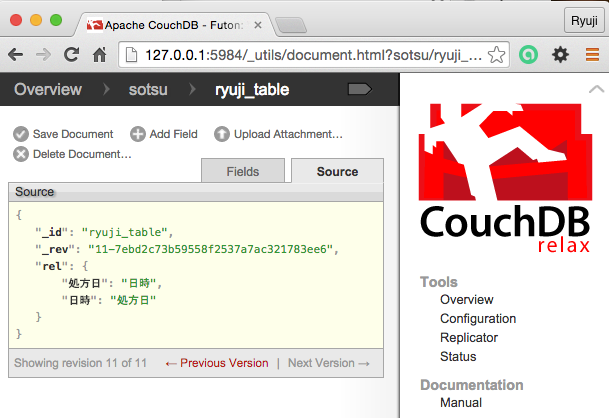
\includegraphics[width=10cm, bb=0 0 609 478, clip]{./gazou/relation2.png}
		\end{center}
		\caption{同義キーを管理するドキュメント}
		\label{relation}
	\end{figure}

	\begin{figure}[htbp]
		\begin{center}
			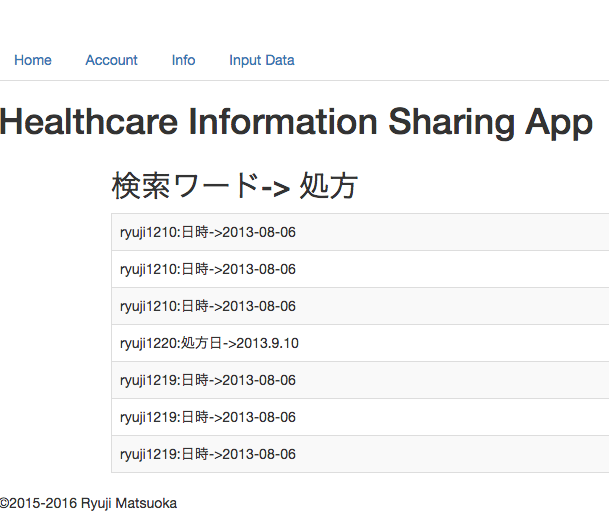
\includegraphics[width=15cm, bb=0 0 609 528, clip]{./gazou/relationApp3.png}
		\end{center}
		\caption{処方と検索して同義キーとして登録されている日時も表示する}
		\label{relationApp}
	\end{figure}


\subsection{NoSQL版のまとめ}
	入力ファイルに対して自由度を持たせながら
	医療情報の閲覧,書き込みをすることができる
	Webアプリケーションを開発することができた.

	既存のものと異なる規格の医療情報入力として受け付ける際,
	以下の3つのものが必要となる.

	\begin{itemize}
		\item そのフォーマットに対するパース処理
		\item データ定義に関する情報
		\item  同義キーの追加登録
	\end{itemize}

	この内, パース処理に関してはパイプ区切りの場合すでに実装しているので,
	改めて必要とはならない.
	また,国内で医療情報共有システムの共通規格が浸透しなくとも,
	項目に対して一意の項目名が設定されれば
	同義キーの追加登録をするのはかかりつけ医が独自に生成した
	ファイルと,一意の項目名との関連付けの分だけで済ませることができる.
	つまり,項目に対して一意の項目名が国内で設定されれば
	それぞれの規格のデータ定義に関する情報だけで
	医療情報共有システムとして運用することができる.
